\chapter{Движение материальной точки в неинерциальной системе координат.
Абсолютное, переносное и относительное движение. Понятие об абсолютной
(полной) и местной (локальной) производных. Формула Бура. Определение
абсолютной скорости и ускорения материальной точки. Кориолисово ускорение.}

\begin{minipage}{.4\textwidth}
    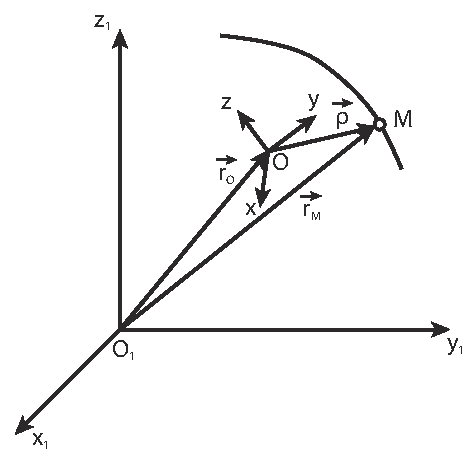
\includegraphics[width=\textwidth]{31_01}
\end{minipage}\hfill
\begin{minipage}{.55\textwidth}
    Абсолютным движением точки называется движение относительно неподвижной
    системы отсчета \( O_1x_1y_1z_1 \).
    
    Относительным движением точки называется движение относительно подвижной
    системы отсчета \( Oxyz \).
    
    Переносным движением точки называется движение точки подвижной системы
    отсчета, с которой в данный момент совпадает движущаяся точка, относительно
    неподвижной системы отсчета.
\end{minipage}

\section{Понятие полной и локальной производных}
Разложим вектор \( \vec{\rho} \) по координатам в подвижной системе \( Oxyz \):
\( \vec{\rho} = x\vec{e}_x + y\vec{e}_y + z\vec{e}_z \).

Производная от него по времени, не учитывающая движение и, следовательно,
изменение ортов \( \vec{e}_x,\ \vec{e}_y,\ \vec{e}_z \) системы со временем,
называется локальной:
\( \ds \widetilde{\der{\vec{\rho}}{t}} = \dot{x}\vec{e}_x + \dot{y}\vec{e}_y +
\dot{z}\vec{e}_z \).

Производная, учитывающая движение системы, называется полной:
\[
    \der{\vec{\rho}}{t} = \dot{x}\vec{e}_x + \dot{y}\vec{e}_y + \dot{z}\vec{e}_z
    + x\der{\vec{e}_x}{t} + y\der{\vec{e}_y}{t} + z\der{\vec{e}_z}{t}.
\]

Обозначая \( \ds \der{\vec{e}_x}{t} = \vec{\omega}\times\vec{e}_x,\ 
\der{\vec{e}_y}{t} = \vec{\omega}\times\vec{e}_y,\ \der{\vec{e}_z}{t} =
\vec{\omega}\times\vec{e}_z \), получим формулу Бура:
\[
    \der{\vec{\rho}}{t} = \widetilde{\der{\vec{\rho}}{t}} + \omega\times\vec{\rho}.
\]
Последнее слагаемое определяет сферическое движение, то есть возникает при
поворотах подвижной системы координат. Вектор \( \vec{\omega} \) называется
мгновенной угловой скоростью подвижной системы координат \( Oxyz \) в
сферическом движении относительно её начала \( O \).

\section{Определение скорости}
Возьмём производную по времени от вектора
\( \vec{r}_M = \vec{r}_O + \vec{\rho} \):
\[
    \der{\vec{r}_M}{t} = \vec{v}_a = \der{\vec{r}_O}{t} + \der{\vec{\rho}}{t} =
    \der{\vec{r}_O}{t} + \widetilde{\der{\vec{\rho}}{t}} +
    \vec{\omega}\times\vec{\rho} = \vec{v}_O + \vec{\omega}\times\vec{\rho} +
    \vec{v}_r = \vec{v}_e + \vec{v}_r,
\]
где \( \ds \vec{v}_a = \der{\vec{r}_M}{t} \) -- абсолютная скорость точки
\( M \), \( \ds\vec{v}_r=\widetilde{\der{\vec{\rho}}{t}} \) -- её относительная
скорость, \( \ds \vec{v}_O =~\der{\vec{r}_O}{t} \) -- абсолютная скорость точки
\( O \), а \( \ds \vec{v}_e = \vec{v}_O + \vec{\omega}\times\vec{\rho} \) --
переносная скорость.

\section{Определение ускорения}
Возьмем производную от скорости по времени:
\begin{align*}
    \der{\vec{v}_a}{t} = \vec{v}_a = \der{\vec{v}_O}{t} +
    \der{\vec{\omega}}{t}\times\vec{\rho} + \vec{\omega}\times
    \der{\vec{\rho}}{t} +\der{\vec{v}_r}{t} = \vec{a}_O + \der{\vec{\omega}}{t}
    \times\vec{\rho} + \vec{\omega}\times\widetilde{\der{\vec{\rho}}{t}} +
    \vec{\omega}\times(\vec{\omega}\times\vec{\rho}) +
    \widetilde{\der{\vec{v}_r}{t}} + \\ + \vec{\omega}\times\vec{v}_r =
    \vec{a}_O + \vec{\eps}\times\vec{\rho} + 2\vec{\omega}\times\vec{v}_r +
    \vec{\omega}\times(\vec{\omega}\times\vec{\rho}) + \vec{a}_r = \vec{a}_O +
    \vec{a}_e^\emph{вр} + \vec{a}_{cor} + \vec{a}_e^\emph{цс} + \vec{a}_r =
    \vec{a}_e + \vec{a}_r + \vec{a}_{cor},
\end{align*}
где \( \ds \vec{a}_a = \der{\vec{v}_a}{t} \) -- абсолютное ускорение точки
\( M \), \( \ds \vec{a}_r = \der{\vec{v}_r}{t} \) -- её относительное ускорение,
\( \vec{a}_{cor} = 2\vec{\omega}\times\vec{v}_r \) -- кориолисово ускорение,
\( \ds \vec{a}_O = \der{\vec{v}_O}{t} \) -- абсолютное ускорение точки \( O \),
\( \vec{a}_e^\emph{цс} = \vec{\omega}\times(\vec{\omega}\times\vec{\rho}) \) --
центростремительное ускорение, \( \vec{a}_e^\emph{вр} = \vec{\eps}\times
\vec{\rho} \) -- вращательное ускорение, \( \ds \vec{\eps} =
\der{\vec{\omega}}{t} \) -- вектор мгновенного углового ускорения.
\newpage
